
%% bare_conf.tex
%% V1.3
%% 2007/01/11
%% by Michael Shell
%% See:
%% http://www.michaelshell.org/
%% for current contact information.
%%
%% This is a skeleton file demonstrating the use of IEEEtran.cls
%% (requires IEEEtran.cls version 1.7 or later) with an IEEE conference paper.
%%
%% Support sites:
%% http://www.michaelshell.org/tex/ieeetran/
%% http://www.ctan.org/tex-archive/macros/latex/contrib/IEEEtran/
%% and
%% http://www.ieee.org/

%%*************************************************************************
%% Legal Notice:
%% This code is offered as-is without any warranty either expressed or
%% implied; without even the implied warranty of MERCHANTABILITY or
%% FITNESS FOR A PARTICULAR PURPOSE! 
%% User assumes all risk.
%% In no event shall IEEE or any contributor to this code be liable for
%% any damages or losses, including, but not limited to, incidental,
%% consequential, or any other damages, resulting from the use or misuse
%% of any information contained here.
%%
%% All comments are the opinions of their respective authors and are not
%% necessarily endorsed by the IEEE.
%%
%% This work is distributed under the LaTeX Project Public License (LPPL)
%% ( http://www.latex-project.org/ ) version 1.3, and may be freely used,
%% distributed and modified. A copy of the LPPL, version 1.3, is included
%% in the base LaTeX documentation of all distributions of LaTeX released
%% 2003/12/01 or later.
%% Retain all contribution notices and credits.
%% ** Modified files should be clearly indicated as such, including  **
%% ** renaming them and changing author support contact information. **
%%
%% File list of work: IEEEtran.cls, IEEEtran_HOWTO.pdf, bare_adv.tex,
%%                    bare_conf.tex, bare_jrnl.tex, bare_jrnl_compsoc.tex
%%*************************************************************************

% *** Authors should verify (and, if needed, correct) their LaTeX system  ***
% *** with the testflow diagnostic prior to trusting their LaTeX platform ***
% *** with production work. IEEE's font choices can trigger bugs that do  ***
% *** not appear when using other class files.                            ***
% The testflow support page is at:
% http://www.michaelshell.org/tex/testflow/



% Note that the a4paper option is mainly intended so that authors in
% countries using A4 can easily print to A4 and see how their papers will
% look in print - the typesetting of the document will not typically be
% affected with changes in paper size (but the bottom and side margins will).
% Use the testflow package mentioned above to verify correct handling of
% both paper sizes by the user's LaTeX system.
%
% Also note that the "draftcls" or "draftclsnofoot", not "draft", option
% should be used if it is desired that the figures are to be displayed in
% draft mode.
%
\documentclass[conference]{IEEEtran}
% Add the compsoc option for Computer Society conferences.
%
% If IEEEtran.cls has not been installed into the LaTeX system files,
% manually specify the path to it like:
% \documentclass[conference]{../sty/IEEEtran}





% Some very useful LaTeX packages include:
% (uncomment the ones you want to load)


% *** MISC UTILITY PACKAGES ***
%
%\usepackage{ifpdf}
% Heiko Oberdiek's ifpdf.sty is very useful if you need conditional
% compilation based on whether the output is pdf or dvi.
% usage:
% \ifpdf
%   % pdf code
% \else
%   % dvi code
% \fi
% The latest version of ifpdf.sty can be obtained from:
% http://www.ctan.org/tex-archive/macros/latex/contrib/oberdiek/
% Also, note that IEEEtran.cls V1.7 and later provides a builtin
% \ifCLASSINFOpdf conditional that works the same way.
% When switching from latex to pdflatex and vice-versa, the compiler may
% have to be run twice to clear warning/error messages.






% *** CITATION PACKAGES ***
%
%\usepackage{cite}
% cite.sty was written by Donald Arseneau
% V1.6 and later of IEEEtran pre-defines the format of the cite.sty package
% \cite{} output to follow that of IEEE. Loading the cite package will
% result in citation numbers being automatically sorted and properly
% "compressed/ranged". e.g., [1], [9], [2], [7], [5], [6] without using
% cite.sty will become [1], [2], [5]--[7], [9] using cite.sty. cite.sty's
% \cite will automatically add leading space, if needed. Use cite.sty's
% noadjust option (cite.sty V3.8 and later) if you want to turn this off.
% cite.sty is already installed on most LaTeX systems. Be sure and use
% version 4.0 (2003-05-27) and later if using hyperref.sty. cite.sty does
% not currently provide for hyperlinked citations.
% The latest version can be obtained at:
% http://www.ctan.org/tex-archive/macros/latex/contrib/cite/
% The documentation is contained in the cite.sty file itself.






% *** GRAPHICS RELATED PACKAGES ***
%
\ifCLASSINFOpdf
  % \usepackage[pdftex]{graphicx}
  % declare the path(s) where your graphic files are
  % \graphicspath{{../pdf/}{../jpeg/}}
  % and their extensions so you won't have to specify these with
  % every instance of \includegraphics
  % \DeclareGraphicsExtensions{.pdf,.jpeg,.png}
\else
  % or other class option (dvipsone, dvipdf, if not using dvips). graphicx
  % will default to the driver specified in the system graphics.cfg if no
  % driver is specified.
  % \usepackage[dvips]{graphicx}
  % declare the path(s) where your graphic files are
  % \graphicspath{{../eps/}}
  % and their extensions so you won't have to specify these with
  % every instance of \includegraphics
  % \DeclareGraphicsExtensions{.eps}
\fi
% graphicx was written by David Carlisle and Sebastian Rahtz. It is
% required if you want graphics, photos, etc. graphicx.sty is already
% installed on most LaTeX systems. The latest version and documentation can
% be obtained at: 
% http://www.ctan.org/tex-archive/macros/latex/required/graphics/
% Another good source of documentation is "Using Imported Graphics in
% LaTeX2e" by Keith Reckdahl which can be found as epslatex.ps or
% epslatex.pdf at: http://www.ctan.org/tex-archive/info/
%
% latex, and pdflatex in dvi mode, support graphics in encapsulated
% postscript (.eps) format. pdflatex in pdf mode supports graphics
% in .pdf, .jpeg, .png and .mps (metapost) formats. Users should ensure
% that all non-photo figures use a vector format (.eps, .pdf, .mps) and
% not a bitmapped formats (.jpeg, .png). IEEE frowns on bitmapped formats
% which can result in "jaggedy"/blurry rendering of lines and letters as
% well as large increases in file sizes.
%
% You can find documentation about the pdfTeX application at:
% http://www.tug.org/applications/pdftex





% *** MATH PACKAGES ***
%
%\usepackage[cmex10]{amsmath}
% A popular package from the American Mathematical Society that provides
% many useful and powerful commands for dealing with mathematics. If using
% it, be sure to load this package with the cmex10 option to ensure that
% only type 1 fonts will utilized at all point sizes. Without this option,
% it is possible that some math symbols, particularly those within
% footnotes, will be rendered in bitmap form which will result in a
% document that can not be IEEE Xplore compliant!
%
% Also, note that the amsmath package sets \interdisplaylinepenalty to 10000
% thus preventing page breaks from occurring within multiline equations. Use:
%\interdisplaylinepenalty=2500
% after loading amsmath to restore such page breaks as IEEEtran.cls normally
% does. amsmath.sty is already installed on most LaTeX systems. The latest
% version and documentation can be obtained at:
% http://www.ctan.org/tex-archive/macros/latex/required/amslatex/math/





% *** SPECIALIZED LIST PACKAGES ***
%
%\usepackage{algorithmic}
% algorithmic.sty was written by Peter Williams and Rogerio Brito.
% This package provides an algorithmic environment fo describing algorithms.
% You can use the algorithmic environment in-text or within a figure
% environment to provide for a floating algorithm. Do NOT use the algorithm
% floating environment provided by algorithm.sty (by the same authors) or
% algorithm2e.sty (by Christophe Fiorio) as IEEE does not use dedicated
% algorithm float types and packages that provide these will not provide
% correct IEEE style captions. The latest version and documentation of
% algorithmic.sty can be obtained at:
% http://www.ctan.org/tex-archive/macros/latex/contrib/algorithms/
% There is also a support site at:
% http://algorithms.berlios.de/index.html
% Also of interest may be the (relatively newer and more customizable)
% algorithmicx.sty package by Szasz Janos:
% http://www.ctan.org/tex-archive/macros/latex/contrib/algorithmicx/




% *** ALIGNMENT PACKAGES ***
%
%\usepackage{array}
% Frank Mittelbach's and David Carlisle's array.sty patches and improves
% the standard LaTeX2e array and tabular environments to provide better
% appearance and additional user controls. As the default LaTeX2e table
% generation code is lacking to the point of almost being broken with
% respect to the quality of the end results, all users are strongly
% advised to use an enhanced (at the very least that provided by array.sty)
% set of table tools. array.sty is already installed on most systems. The
% latest version and documentation can be obtained at:
% http://www.ctan.org/tex-archive/macros/latex/required/tools/


%\usepackage{mdwmath}
%\usepackage{mdwtab}
% Also highly recommended is Mark Wooding's extremely powerful MDW tools,
% especially mdwmath.sty and mdwtab.sty which are used to format equations
% and tables, respectively. The MDWtools set is already installed on most
% LaTeX systems. The lastest version and documentation is available at:
% http://www.ctan.org/tex-archive/macros/latex/contrib/mdwtools/


% IEEEtran contains the IEEEeqnarray family of commands that can be used to
% generate multiline equations as well as matrices, tables, etc., of high
% quality.


%\usepackage{eqparbox}
% Also of notable interest is Scott Pakin's eqparbox package for creating
% (automatically sized) equal width boxes - aka "natural width parboxes".
% Available at:
% http://www.ctan.org/tex-archive/macros/latex/contrib/eqparbox/





% *** SUBFIGURE PACKAGES ***
%\usepackage[tight,footnotesize]{subfigure}
% subfigure.sty was written by Steven Douglas Cochran. This package makes it
% easy to put subfigures in your figures. e.g., "Figure 1a and 1b". For IEEE
% work, it is a good idea to load it with the tight package option to reduce
% the amount of white space around the subfigures. subfigure.sty is already
% installed on most LaTeX systems. The latest version and documentation can
% be obtained at:
% http://www.ctan.org/tex-archive/obsolete/macros/latex/contrib/subfigure/
% subfigure.sty has been superceeded by subfig.sty.



%\usepackage[caption=false]{caption}
%\usepackage[font=footnotesize]{subfig}
% subfig.sty, also written by Steven Douglas Cochran, is the modern
% replacement for subfigure.sty. However, subfig.sty requires and
% automatically loads Axel Sommerfeldt's caption.sty which will override
% IEEEtran.cls handling of captions and this will result in nonIEEE style
% figure/table captions. To prevent this problem, be sure and preload
% caption.sty with its "caption=false" package option. This is will preserve
% IEEEtran.cls handing of captions. Version 1.3 (2005/06/28) and later 
% (recommended due to many improvements over 1.2) of subfig.sty supports
% the caption=false option directly:
%\usepackage[caption=false,font=footnotesize]{subfig}
%
% The latest version and documentation can be obtained at:
% http://www.ctan.org/tex-archive/macros/latex/contrib/subfig/
% The latest version and documentation of caption.sty can be obtained at:
% http://www.ctan.org/tex-archive/macros/latex/contrib/caption/




% *** FLOAT PACKAGES ***
%
%\usepackage{fixltx2e}
% fixltx2e, the successor to the earlier fix2col.sty, was written by
% Frank Mittelbach and David Carlisle. This package corrects a few problems
% in the LaTeX2e kernel, the most notable of which is that in current
% LaTeX2e releases, the ordering of single and double column floats is not
% guaranteed to be preserved. Thus, an unpatched LaTeX2e can allow a
% single column figure to be placed prior to an earlier double column
% figure. The latest version and documentation can be found at:
% http://www.ctan.org/tex-archive/macros/latex/base/



%\usepackage{stfloats}
% stfloats.sty was written by Sigitas Tolusis. This package gives LaTeX2e
% the ability to do double column floats at the bottom of the page as well
% as the top. (e.g., "\begin{figure*}[!b]" is not normally possible in
% LaTeX2e). It also provides a command:
%\fnbelowfloat
% to enable the placement of footnotes below bottom floats (the standard
% LaTeX2e kernel puts them above bottom floats). This is an invasive package
% which rewrites many portions of the LaTeX2e float routines. It may not work
% with other packages that modify the LaTeX2e float routines. The latest
% version and documentation can be obtained at:
% http://www.ctan.org/tex-archive/macros/latex/contrib/sttools/
% Documentation is contained in the stfloats.sty comments as well as in the
% presfull.pdf file. Do not use the stfloats baselinefloat ability as IEEE
% does not allow \baselineskip to stretch. Authors submitting work to the
% IEEE should note that IEEE rarely uses double column equations and
% that authors should try to avoid such use. Do not be tempted to use the
% cuted.sty or midfloat.sty packages (also by Sigitas Tolusis) as IEEE does
% not format its papers in such ways.





% *** PDF, URL AND HYPERLINK PACKAGES ***
%
%\usepackage{url}
% url.sty was written by Donald Arseneau. It provides better support for
% handling and breaking URLs. url.sty is already installed on most LaTeX
% systems. The latest version can be obtained at:
% http://www.ctan.org/tex-archive/macros/latex/contrib/misc/
% Read the url.sty source comments for usage information. Basically,
% \url{my_url_here}.





% *** Do not adjust lengths that control margins, column widths, etc. ***
% *** Do not use packages that alter fonts (such as pslatex).         ***
% There should be no need to do such things with IEEEtran.cls V1.6 and later.
% (Unless specifically asked to do so by the journal or conference you plan
% to submit to, of course. )

\usepackage{graphicx}
\graphicspath{{./figures/}}


% correct bad hyphenation here
\hyphenation{op-tical net-works semi-conduc-tor}


\begin{document}
%
% paper title
% can use linebreaks \\ within to get better formatting as desired
\title{Real-time Hermite Polynomial Characterization of Heartbeats using a Field-Programmable Gate Array}


% author names and affiliations
% use a multiple column layout for up to three different
% affiliations
%\author{\IEEEauthorblockN{Kartik Lakhotia}
%\IEEEauthorblockA{Indian Institute of Technology (Bombay),\\
%Powai, Mumbai 400076, India\\\\
%Email: kartik@ee.iitb.ac.in}
%\and
%\IEEEauthorblockN{Gabriel Caffarena}
%\IEEEauthorblockA{Twentieth Century Fox\\
%Springfield, USA\\
%Email: homer@thesimpsons.com}
%\and
%\IEEEauthorblockN{Alberto Gil}
%\IEEEauthorblockA{Starfleet Academy\\
%San Francisco, California 96678-2391\\
%Telephone: (800) 555--1212\\
%Fax: (888) 555--1212}}

% conference papers do not typically use \thanks and this command
% is locked out in conference mode. If really needed, such as for
% the acknowledgment of grants, issue a \IEEEoverridecommandlockouts
% after \documentclass

% for over three affiliations, or if they all won't fit within the width
% of the page, use this alternative format:
% 

\author{\IEEEauthorblockN{Kartik Lakhotia\IEEEauthorrefmark{1},
Gabriel Caffarena\IEEEauthorrefmark{2},
Alberto Gil\IEEEauthorrefmark{2}, 
David G. M\'{a}rquez\IEEEauthorrefmark{3},
Abraham Otero\IEEEauthorrefmark{2} and 
Madhav P. Desai \IEEEauthorrefmark{1}}
\IEEEauthorblockA{\IEEEauthorrefmark{1}Indian Institute of Technology (Bombay)\\
Powai, Mumbai 400076, India\\
Email: madhav@ee.iitb.ac.in}
\IEEEauthorblockA{\IEEEauthorrefmark{2}Laboratory of Bioengineering\\
University CEU-San Pablo, Boadilla del Monte 28668, Spain\\
Email: gabriel.caffarena@ceu.es}
\IEEEauthorblockA{\IEEEauthorrefmark{3}Centro Singular de Investigacion en Tecnologias da Informacion (CITIUS)\\
University of Santiago de Compostela, 15782 Santiago de Compostela, Spain\\
Email: david.gonzalez.marquez@usc.es}}




% use for special paper notices
%\IEEEspecialpapernotice{(Invited Paper)}




% make the title area
\maketitle


\begin{abstract}
%\boldmath
The characterization of ECG heartbeats is a computationally intensive problem, and
both off-line and on-line (real-time) solutions to this problem are of great interest.
In this paper, we consider the use of a dedicated hardware implementation
(using a field-programmable gate-array (FPGA)) to solve a critical component of this problem,
namely,  the best-fit Hermite approximation of a heartbeat.
The implementation is generated using an algorithm-to-hardware compiler tool-chain
and the resulting hardware is characterized using an off-the-shelf FPGA card.
The single beat best-fit computation latency when using six Hermite basis
polynomials is under $0.5ms$ with a power dissipation of 3 watts, demonstrating
true real-time applicability. 
\end{abstract}
% IEEEtran.cls defaults to using nonbold math in the Abstract.
% This preserves the distinction between vectors and scalars. However,
% if the conference you are submitting to favors bold math in the abstract,
% then you can use LaTeX's standard command \boldmath at the very start
% of the abstract to achieve this. Many IEEE journals/conferences frown on
% math in the abstract anyway.

The characterization of ECG heartbeats is a computationally intensive problem, and
both off-line and on-line (real-time) solutions to this problem are of great interest.
In this paper, we consider the use of a dedicated hardware implementation
(using a field-programmable gate-array (FPGA)) to solve a critical component of this problem. 
We describe an implementation of real-time best-fit Hermite approximation of a heartbeat using six Hermite polynomials.  
The implementation is generated using an algorithm-to-hardware compiler tool-chain
and the resulting hardware is characterized using an off-the-shelf FPGA card.
The single beat best-fit computation latency is under $0.5ms$ with a power dissipation of 3 watts.

% no keywords




% For peer review papers, you can put extra information on the cover
% page as needed:
% \ifCLASSOPTIONpeerreview
% \begin{center} \bfseries EDICS Category: 3-BBND \end{center}
% \fi
%
% For peerreview papers, this IEEEtran command inserts a page break and
% creates the second title. It will be ignored for other modes.
\IEEEpeerreviewmaketitle



Automatic ECG analysis and characterization can be of great help
in patient monitoring.
In particular, the characterization of the QRS complex by means of Hermite functions 
seems to be a reliable mechanism  for automatic classification of heartbeats \cite{j:lagerholm00}. 
The main advantages seem to be the low sensitivity to noise and artifacts, and the
compactness of the representation (e.g. a 144-sample QRS can be characterized with 7 parameters \cite{c:marquez13}). 
These advantages have made the Hermite representation a very common tool for characterizing the 
morphology of the beats \cite{j:lagerholm00,c:marquez13,c:braccini97,j:linh03a,j:linh03b}. 

ECG analysis using Hermite functions has a
substantial amount of parallelism.  Solutions to the problem have been investigated
using processors (and multi-cores) and graphics processing units (GPU's). 
In this paper, we consider the alternative route of using an FPGA to implement
the computations.  In particular, our work is motivated by the potential
of an FPGA (or eventually, a dedicated application-specific circuit) for low-latency
energy efficient heart-beat analysis.  

In generating the hardware for heart-beat analysis, we make extensive use of
algorithm-to-hardware techniques.  By this we mean that the hardware is
generated from an algorithmic specification that is written in a
high-level programming language ({\bf C} in this case), which is then
transformed to a circuit implementation using the AHIRV2 algorithm to hardware 
compilation tools \cite{c:ahir_thesis2009,c:ahir_dsd2010,c:ahir_usenix2012}.
The resulting hardware is then mapped to an FPGA card (the ML605 card from Xilinx,
which uses a Virtex-6 FPGA).  The circuit is then exercised through the PCI-express 
interface and used to classify beats.  The round-trip latency of a single
beat classification was found to be under $0.5ms$.


\section{QRS approximation by means of Hermite polynomials}\label{s:arr}

The aim of using the Hermite approximation to estimate heartbeats is to 
reduce the number of dimensions required to carry out the ECG classification, 
without sacrificing accuracy. 
The benchmarks used in this work come from the MIT-BIH arrhythmia database \cite{j:moody01} which is made up of 
48 ECG recordings whose beats  have been manually annotated by two cardiologists. 
Each file from the database 
contains 2 ECG channels, sampled at a frequency of 360 Hz and with a duration of approximately 2000 beats. 

Before doing the Hermite approximation, the ECG signal is processed to remove
the base-line drift.  The QRS complexes for each heartbeat are extracted by 
finding the peak of the beat (e.g. the R wave) and selecting a  window of 200 ms centered on the peak. 
The beat-window is further extended to 400 ms by padding 100-ms sequences of zeros at each side of the complex. 
Thus, the QRS beat data used as an input to the Hermite polynomial approximation
consists of individual beats described as a 144-sample vector $\vec{x}=\{x(t)\}$ of double
precision floating point numbers. 
This vector is to be estimated with a linear combination of $N$ Hermite basis functions (for
the work reported in this paper, we use $N=6$).

The goal then is to find the best minimum-mean-square-error (MMSE)  approximation to
$\{ x(t)\}$ as 
\begin{equation}\label{eqn:hat}
\hat{x}(t)=\sum_{n=0}^{N-1}c_n(\sigma )\phi_n(t,\sigma),
\end{equation}

\noindent with

\begin{equation}\label{eqn:phi}
\phi_n(t,\sigma )=\frac{1}{\sqrt{\sigma 2^n n!\sqrt{\pi}}}e^{-t^2/2\sigma^2}H_n(t/\sigma) 
\end{equation}

\noindent where $H_n(t/\sigma)$ is the $n^{th}$ Hermite polynomial. 
These polynomials can be computed recursively as

\begin{equation}
H_n(x)=2xH_{n-1}(x)-2(n-1)H_{n-2}(x),
\end{equation}

\noindent where $H_0(x)=1$ and $H_1(x)=2x$.
The parameter $\sigma$ is a time-scaling factor in the polynomials which needs
to be chosen carefully.   In \cite{j:lagerholm00} the maximum value 
of $\sigma$ for a given order $n$ is estimated.  As the value of $n$ increases, the value of $\sigma_{MAX}$ decreases.

The Hermite polynomials are orthonormal.  Thus, the optimal coefficients that 
minimize the estimation error for a given $\sigma$ are

\begin{equation}\label{eqn:c}
c_n(\sigma)=\sum_{t} x(t)\cdot \phi_n(t,\sigma) 
\end{equation}

The best fit is calculated by comparing the MMSE approximation for each $\sigma$, and keeping
the one with the smallest value.
Once the best $\sigma$ and the corresponding fit coefficients $\vec{c}=\{c_n(\sigma)\}$  \mbox{$(n\in [0,N-1])$} 
are found for each heartbeat, it is possible to use only these figures to perform morphological 
classification of the heartbeats \textrm{~\cite{j:lagerholm00}}.


\section{Beginning the FPGA implementation: the algorithm} \label{s:algorithm}

The algorithm used in the FPGA implementation is illustrated in 
Figure \ref{fig:FpgaAlgo}.
\begin{figure}
\begin{centering}
\small\begin{verbatim}
void HermiteBestFit()
{  
    receiveHermiteBasisFunctions();

    while(1)
    {
        receiveHeartBeat();
        innerProducts();
        findBestFit();
        reportResults();
    }
}
\end{verbatim}
\normalsize
\end{centering}
\caption{High-level view of algorithm mapped to the FPGA}
\label{fig:FpgaAlgo}
\end{figure}

The implementation first receives the values of the Hermite polynomial basis
functions, and  stores them in distinct arrays in the hardware.  In the
current implementation, we use six
arrays to store the basis functions for order $n=0$ to $n=5$.  For each
$n$, basis functions for ten different values of $\sigma$ are stored in the corresponding
array.  The values of $\sigma$ used range from $1/120$ to $1/90$.

After this initialization step, the hardware executes a continuous loop.  
In the loop body, the hardware first listens for heart beats. When
a complete heart-beat (144 samples) is received, the inner products of the
heart-beat with all the basis functions are calculated in a double loop.  
After all inner products are calculated, the inner product coefficients
are used to compute the best fit among the different values of $\sigma$.
The best-fit $\sigma$ index and coefficients
%fitted values 
are then written out of the hardware. 

The algorithm as described above is purely sequential
and does not contain any explicit parallelization.  The AHIRV2 compiler
(described later in Section \ref{s:AHIRV2}) is intelligent enough to extract 
parallelism from the two critical loops (in the inner-product and best-fit functions).
Even with this simple coding of the hardware algorithm,
we observe that excellent real-time performance
is observed (in comparison with CPU/GPU implementations).
Going further, it is possible to specify explicit parallelism by
and exploit it by using multiple function units in hardware
in order to reduce the processing latency.  These investigations
are currently in progress.



\subsection{The inner product loop} \label{sec:InnerProduct}

\begin{figure}
\begin{centering}
\small\begin{verbatim}
void  innerProduct()
{
  int I;
  for (I=0; I < NSAMPLES; I++)
  { // outer-loop
     double x = inputData[I];
     for(SI = 0; SI < NSIGMAS; SI++)
     { // inner-loop
        int I0 = I + Offset[SI];
        double p0 = (x*hF0[I0]);
        double p1 = (x*hF1[I0]);
        double p2 = (x*hF2[I0]);
        double p3 = (x*hF3[I0]);
        double p4 = (x*hF4[I0]);
        double p5 = (x*hF5[I0]);
        dotP0[SI] += p0;
        dotP1[SI] += p1;
        dotP2[SI] += p2;
        dotP3[SI] += p3;
        dotP4[SI] += p4;
        dotP5[SI] += p5;
     }
}
\end{verbatim}
\normalsize
\end{centering}
\caption{Inner-product loop}
\label{fig:InnerProduct}
\end{figure}

The inner product loop is shown in Figure \ref{fig:InnerProduct}.
The outer loop is over the samples, and the inner
loop across the $\sigma$ values.  There is a high-level
of parallelism in the inner loop which can be further
boosted by unrolling the outer loop.   When translating
this to hardware, the entire function uses one single double-precision
multiplier and one single double-precision adder.  Further
note that the arrays $hFn$ and $dotPn$ are declared on
a per-$n$ basis (for $n=0$ to $n=5$). This allows the arrays to be mapped to
distinct memory spaces, thus increasing the memory access bandwidth in the hardware.

\subsection{The minimum-mean-square loop} \label{sec:MMSE}

\begin{figure}
\begin{centering}
\footnotesize\begin{verbatim}
void computeMSE()
{
  int I, SI;
  best_mse = 1.0e+20;
  best_sigma_index = -1;
  for (I=0; I<NSAMPLES; I=I+4)
  { // outer-loop
     for (SI=0; SI<NSIGMAS; SI++)
     { // inner-loop
        int fetchIndex0 = I + Offset[SI]; 
        double p0 = (dotP0[SI]*hF0[fetchIndex0]);
        double p1 = (dotP1[SI]*hF1[fetchIndex0]);
        double p2 = (dotP2[SI]*hF2[fetchIndex0]);
        double p3 = (dotP3[SI]*hF3[fetchIndex0]);
        double p4 = (dotP4[SI]*hF4[fetchIndex0]);
        double p5 = (dotP5[SI]*hF5[fetchIndex0]);
        double diff = (inputData[I]-
                      ((p0+p1) + (p2+p3) + (p4+p5)));
        err[SI] += (diff*diff);
      }
    }
    for (SI=0; SI<NSIGMAS; SI++)
    {
        if(err[SI] <  best_mse)
        {
           best_mse = err[SI];
           best_sigma_index = SI;
        }
    }
}
\end{verbatim}
\normalsize
\end{centering}
\caption{MMSE calculation loop}
\label{fig:MMSE}
\end{figure}


The MMSE calculation hardware
uses the algorithm shown in Figure \ref{fig:MMSE}.
Note that the inner loop again has considerable parallelism.
One pipelined double precision multiplier and one
pipelined double precision adder are used to implement
the loop.  The arrays referred to in the loop
$dotPn$ and $hFn$ are all implemented in disjoint
memories to give high memory access bandwidth.



\subsection{Optimizations: loop unrolling and loop pipelining}

The current implementation uses a simple sequential specification.
We have investigated the impact of
further optimizations.  In particular, we find that outer-loop
unrolling (up to four) and inner-loop pipelining 
have substantial impact on the performance of the generated hardware.

If we look at the inner loop in Figure \ref{fig:InnerProduct},
we observe that because of the accumulation of products in each
loop iteration, the time interval between successive loop initiations
is equal to the latency of the adder (because the next loop iteration
needs to wait for the completion of the sum in the current iteration).  This
latency is around 20 cycles in our case, and becomes a performance limiter.

If the outer loop in the innner-product function
(Section \ref{sec:InnerProduct}) is unrolled four times, the 
resulting code will have the form shown in Figure \ref{fig:InnerProductUnrolled}.
The amount of parallelism in the inner loop increases by a considerable
margin.  The loop iteration initiation latency stays about the same, but the
amount of computation done in each loop iteration is quadrupled, thus
leading to higher performance.  In Section \ref{s:results}, we
provide actual measurements in hardware which support this observation.

A similar improvement is observed by unrolling the outer loop in the MMSE computation
shown in Figure \ref{fig:MMSE}.

\begin{figure}
\begin{centering}
\small\begin{verbatim}
void  innerProduct()
{
  for (I=0; I < NSAMPLES; I += 4)
  { // outer-loop
     double x0 = inputData[I];
     double x1 = inputData[I+1];
     double x2 = inputData[I+2];
     double x3 = inputData[I+3];
     for(SI = 0; SI < NSIGMAS; SI++)
     { 
        int I0 = I + Offset[SI];
        I1 = I0+1; I2 = I0+2; I3 = I0+3;
        // compute inner product of 
        // (x0,x1,x2,x3) with
        // (hFn[I0], hFn[I1], hFn[I2], hFn[I3])
        // for n=0,1,2,..5.
        // 
        // accumulate into dotPn[SI].
        //
     }
}
\end{verbatim}
\normalsize
\end{centering}
\caption{Inner-product loop unrolled four times.}
\label{fig:InnerProductUnrolled}
\end{figure}


\section{From algorith-to-hardware using AHIRV2, a C-2-VHDL compiler} \label{s:AHIRV2}
%%(Madhav, reuse some text and figures from other publications to explain AHIR methodology. 
%% Also, it would be interesting to mention the way that AHIR handles data types (int and float)
%%
The AHIRV2 compiler tool-chain \cite{c:ahir_thesis2009, c:ahir_dsd2010, c:ahir_usenix2012} 
provides a pathway from a C-program to actual synthesizable hardware.  The tool-chain
takes a description of an algorithm (described in C) and produces a VHDL logic circuit
description which is equivalent to the algorithm.

The AHIRV2 compiler starts with a C program and produces VHDL.  For the
The clang-2.8 compiler\footnote{www.clang.org} is used as the C front-end
and is used to emit LLVM byte-code\footnote{www.llvm.org}, 
which is then transformed to VHDL using the following transformations:
\begin{enumerate}
\item The LLVM byte-code is translated to an internal intermediate
format, which is itself a static-single assignment centric 
control-flow language (named {\bf Aa}) which allows the description of parallelism
using fork-join structures as well as arbitrary branching.
\item The {\bf Aa} description is translated to a virtual circuit (the model
is described in the next section).  During this translation, the
following major optimizations
are performed:  declared storage objects are partitioned into disjoint memory
spaces using pointer reference analysis, and dependency analysis is used to
generate appropriate sequencing of operations in order to maximize the 
parallelism.  Inner loops in the {\bf Aa} code are pipelined so that
multiple iterations of a loop can be executed concurrently.  
\item The virtual circuit is then translated to VHDL.  At this point,
decisions about operator sharing are taken.  Concurrency analysis is
used to determine if a shared hardware unit needs arbitration. Optimizations
related to clock-frequency maximization are also carried out here.
The generated VHDL uses a pre-designed library of useful operators ranging from
multiplexors, arbiters to pipelined floating point arithmetic units (arbitrary
precision arithmetic is supported, and in particular, there is
full support for IEEE-754 single precision and double precision add/multiply with
all rounding modes).
\end{enumerate}


\subsection{An illustration of the virtual circuit generated by the AHIRV2 compiler}

The virtual circuit generated by the AHIRV2 compiler consists of three
cooperating components: the control-path, the data-path and
the storage system \cite{c:ahir_dsd2010,c:ahir_usenix2012}.

To illustrate the model, we consider a simple example.
\begin{verbatim}
float a[1024], b[1024];
float dotp = 0.0;
for(i=0; i < 1024; i++)
{
   dotp += a[i]*b[i];
}
\end{verbatim}
The AHIRV2 tool-chain transforms this program to 
produce a virtual circuit which is depicted in Figure \ref{fig:dotP}. The
virtual circuit is then translated to synthesizable VHDL.
The virtual circuit consists of three components independent parts, namely
the data-path, the storage-subsystem and the control-path.

\begin{figure*}[ht]
  \centering
  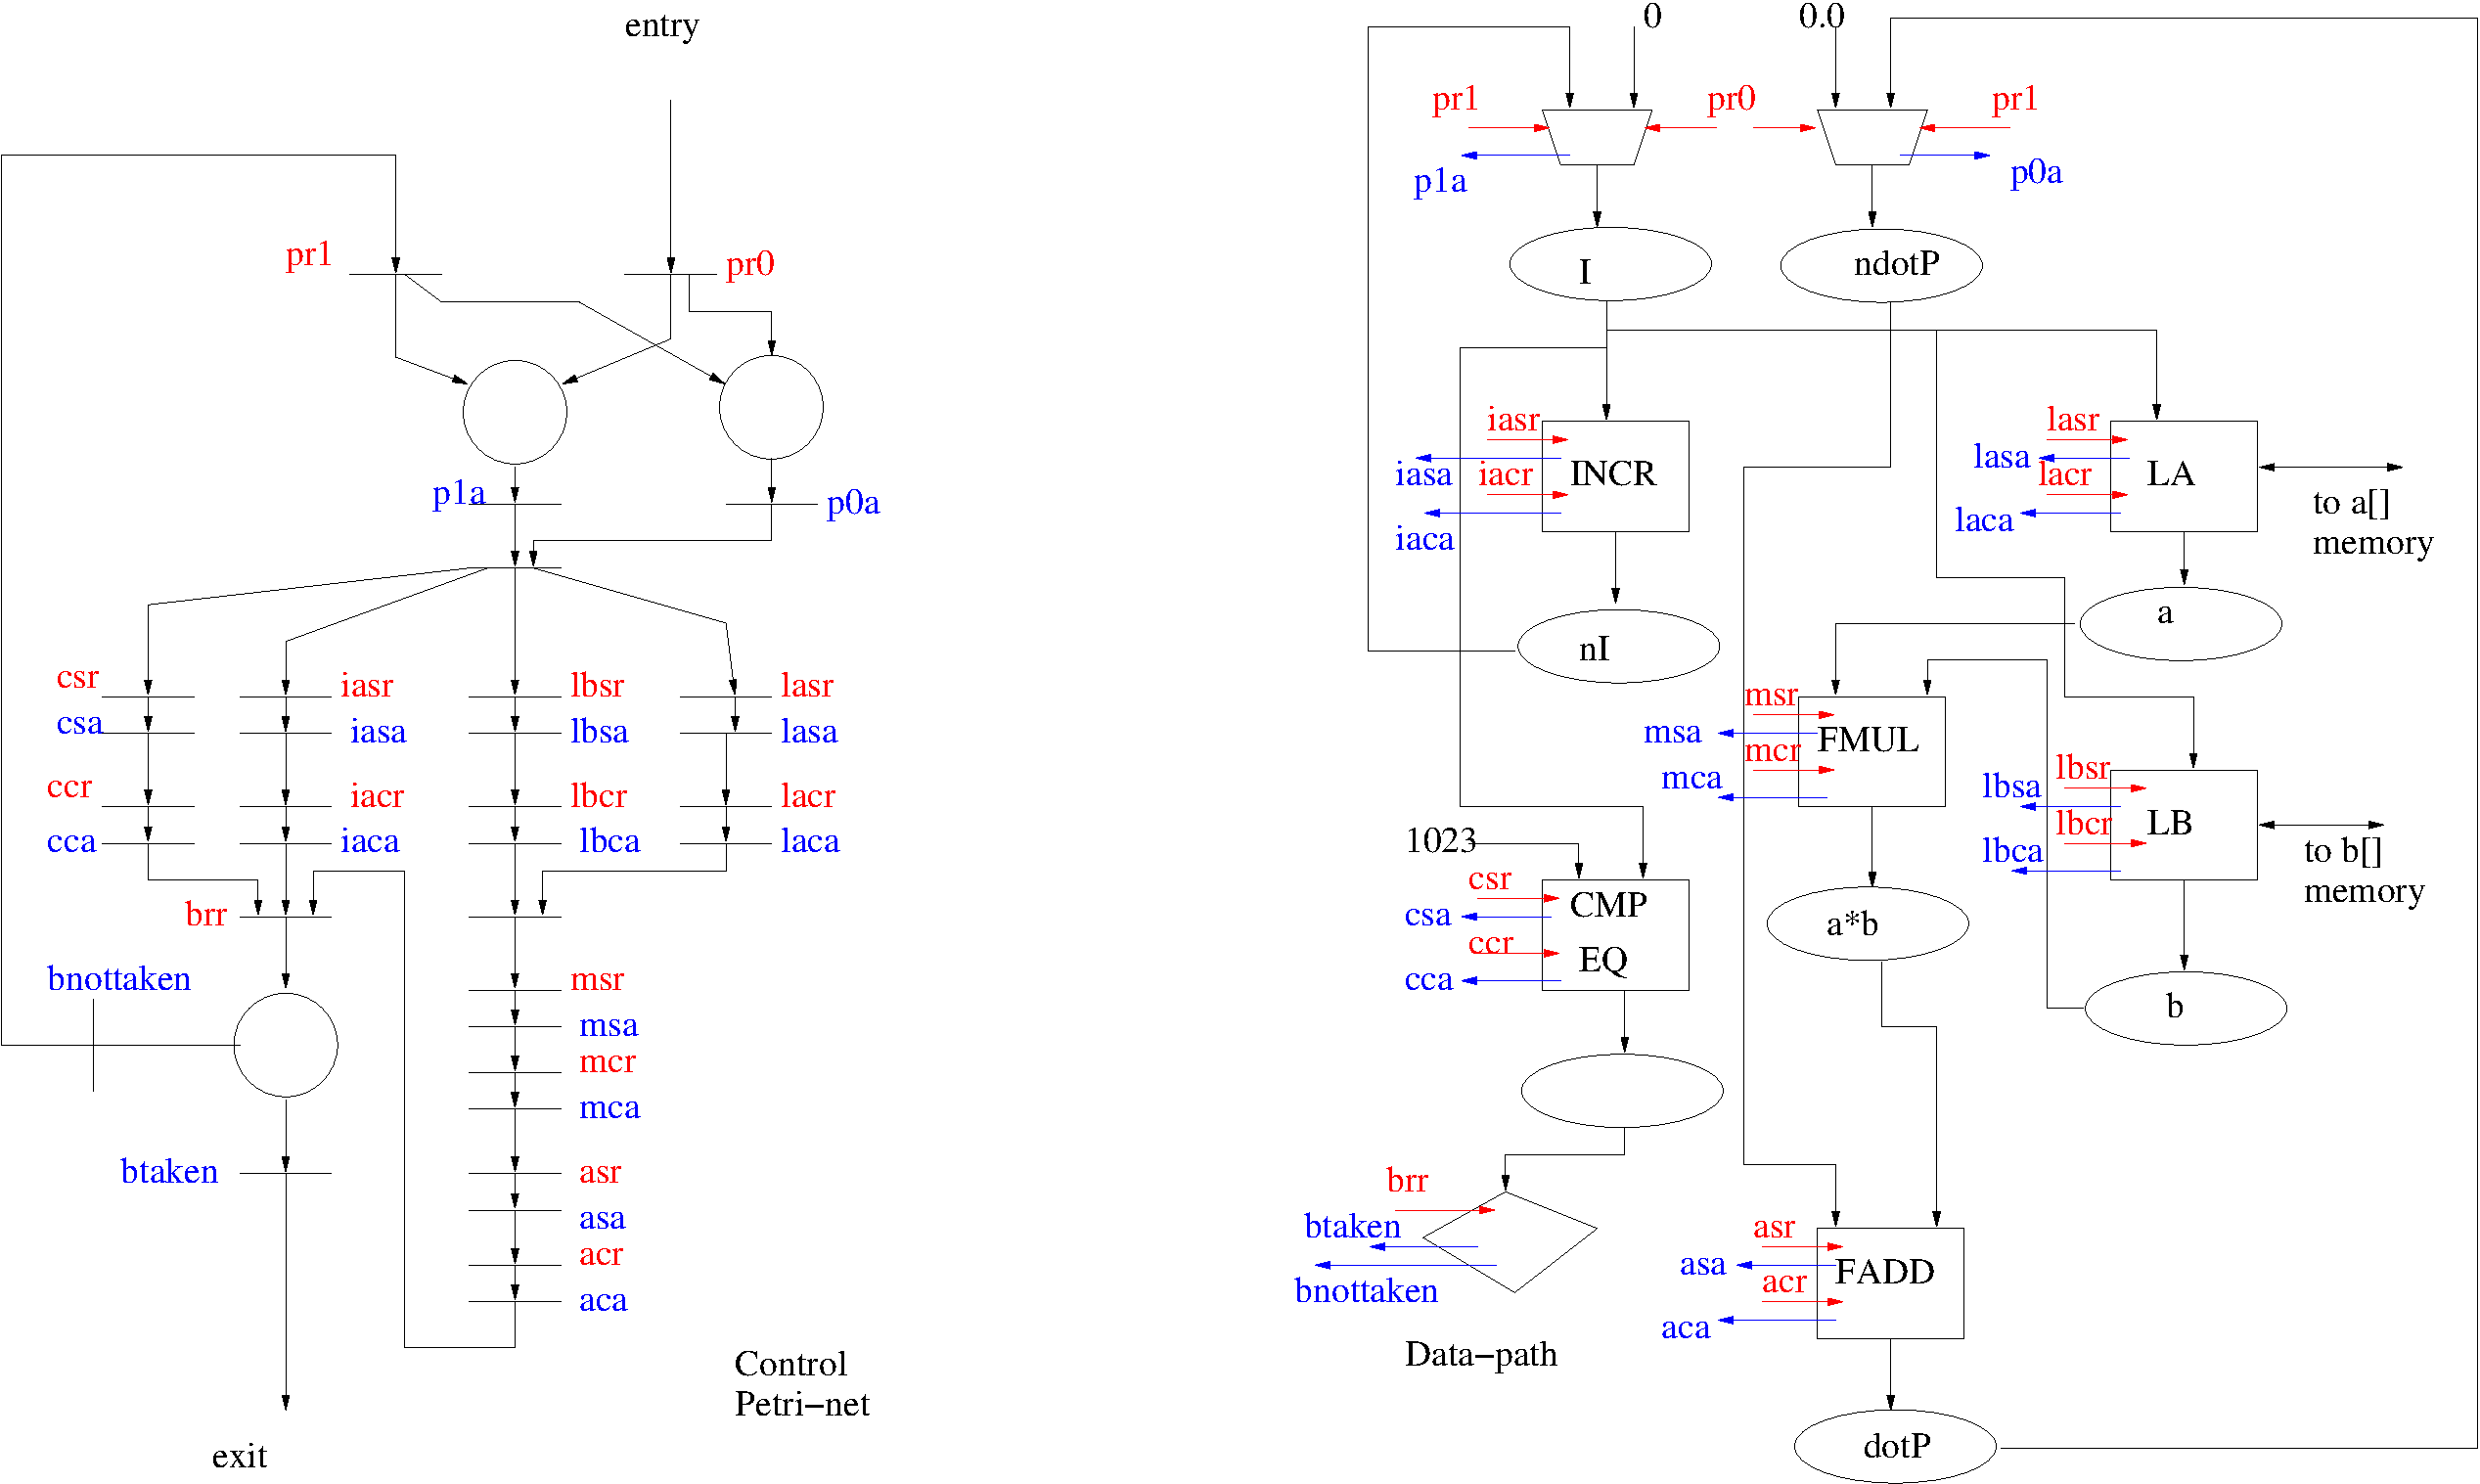
\includegraphics[width=\linewidth]{dotP.pdf}
  \caption{Control-data-storage virtual circuit model.}
  \label{fig:dotP}
\end{figure*}



\subsubsection{The data-path}

The data-path is a directed hyper-graph with nodes being
operations and arcs being nets (shown as ovals).  Each
net has at most one operation which drives it.  Further, most
operations have  a split protocol handshake with
the control-path:  two pairs of request/acknowledge 
associations (*sr/*sa for sampling the inputs  and *cr/*ca for
updating the outputs).    The operation samples its inputs
on receiving the sr request symbol and acknowledges the completion
of this action by emitting the sa acknowledge symbol.  After receiving
the cr symbol, the operation will update its output net
using the newly computed value. The sequencing is required to be
\begin{verbatim}
sr -> sa -> cr -> ca
\end{verbatim}
Note that an operation can be re-triggered while an earlier
edition of the operation
is in progress (this is important if the operation is implemented
using a pipelined operator).

Some data-path operations (such as the multiplexor
shown on the top and the decision operation shown at the bottom
left in Figure \ref{fig:dotP}) follow a simpler protocol.  The multiplexor
has a pair of requests and a single acknowledge, with the condition
that at most one of the requests is received at any time instant.
The input corresponding to the request is then sampled and stored
in the output net of the multiplexor.
The decision operation has a single request and two acknowledes.  Upon
receipt of the request symbol, the decision operation checks its input net
and emits one of the two acknowledges depending on whether the input
is zero/non-zero.

In Figure \ref{fig:dotP}, the following data-path operations
are instantiated:
\begin{verbatim}
mI, mdotP  multiplexors for I, dotP.
INCR       increment for I++
LA         load for a[I]
LB         load for b[I]
FMUL       multiply for p=a[I]*b[I]
FADD       add for dotP += a*b
CMP EQ     compare for COND=(I==1023)
D          decision  COND?
\end{verbatim}


\noindent
{\bf Remark}
Note that the data-path only shows the operations and their interconnection.
When the data-path is implemented as hardware, multiple operations may
be mapped to a single operator depending on cost/performance tradeoffs.  When
this is done, multiplexing logic is introduced in the hardware.  These
decisions and manipulations are performed in the compiler stage which is
responsible for transforming the virtual circuit to VHDL.

\subsubsection{Storage subsystem}

%%
%% time-stamping scheme, in order completion.
%%
The load and store operations in the data-path
are associated with memory subsystems.  In general, there
can be multiple disjoint memory subsystems inferred by the
compiler.  In this particular case, the arrays a[] and b[] 
are mapped to disjoint memories, due to which the two
loads are allowed to proceed in parallel (the relaxed consistency
model is enforced).
In order to maintain the relaxed consistency model, the
memory subsystems are designed to use a time-stamping 
scheme which guarantees first-come-first-served access to
the same memory location.

\subsubsection{Control-path}
%%
%%  control path and data-flow
%%


%% 
%% Petri-net, constructed according to
%% certain rules.  Req/Ack transitions
%%
The control-path in the virtual circuit encodes
all the sequencing that is necessary for correct
operation of the assembly.
The control-path (shown on the left
in Figure \ref{fig:dotP}) is modeled as a Petri-net with
a unique entry point and a unique exit point.  The Petri-net
is constructed using a set of production rules which guarantee
liveness and safeness \cite{c:ahir_dsd2010}.  Transitions in the Petri-net
are associated with output symbols to the data-path (these can
be described by the regular expressions *sr and *cr)
and input symbols from the data-path (these are of the form *sa and
*ca).  The *sr symbols instruct an element in the data-path to
sample its inputs and the *cr symbols instruct an element in the
data-path to update its outputs (all outputs of data-path elements
are registered).  The *sa and *ca symbols are acknowledgements
from the data-path which indicate that the corresponding requests
have been served.  

The following classes of dependencies are
encoded in the control Petri-net:
\begin{itemize}
\item Read-after-write (RAW):  If the result of operator A is used
as an input to operator B, the sr symbol to B can be emitted only after
the ca symbol from A has been received.
\item Write-after-read (WAR): If B writes to a net whose value needs
to have been used by A earlier, for example as in
\begin{verbatim}
a = (b+c) -- operation A reads c
c = (p*q) -- operation B writes to c
\end{verbatim}
where there is a WAR dependency through c,
 then the cr request to B can be
issued only after the sa acknowledge from A has been received.
\item Load-Store ordering:  If P,Q are load/store operations
to the same memory subsystem, and if at least one of P,Q is a
store, and if P is supposed to happen before Q,  then the sr request
to Q must be emitted only after the sa acknowledge from Q
has been received.  The memory subsystem itself guarantees
that requests finish in the same order that they were
initiated.  This takes care of WAR, RAW and WAW memory
dependencies.
\end{itemize}

The control-path in Figure \ref{fig:dotP} shows the sequencing
generated by these rules.  When pipelining an inner loop,
the execution of an operation in a particular iteration is
enabled as soon as its dependencies on results from previous
iterations are satisfied.  


\section{Hardware Implementation Details}\label{s:implementation}

The overall system has 3 major components:
\begin{itemize}
\item A host computer, which is used to calculate the Hermite basis functions,
initialize the FPGA card, send beat data to the FPGA card and receive
the best-fit coefficients from the FPGA card.
\item The FPGA card, on which the best-fit algorithm is implemented.   We use the
Xilinx ML605 card which features a Virtex-6 FPGA and an 8-lane PCI express interface.
\item The FPGA card driver, which is based on the RIFFA infrastructure \cite{c:jacobsen13}. 
\end{itemize}

The algorithm mapped to the FPGA 
is first described in a C program (code fragments descibed in Sections \ref{s:algorithm},  \ref{sec:InnerProduct} and \ref{sec:MMSE}).
The architecture of the hardware produced is shown in Figure \ref{fig:HardwareArchitecture}.
In the initialization phase, the hardware-side listens on an input FIFO to acquire
the Hermite polynomials (these are stored in six disjoint memories, one
for each order $n=0,1,2,\ldots 5$).  After this step, the unit that receives
the beat samples is triggered.  This unit listens on the input FIFO and receives a 144 sample
heartbeat (coded as 144 double-precision floating point numbers).  After receiving
the sample, it triggers the inner-product stage.  In the inner-product stage, the hardware computes, for each $\sigma$ and
$n$, an inner product of the received beat with the Hermite polynomials $\phi_n(t,\sigma)$.
We are using ten values of $\sigma$ and $6$ values of $n$.  Thus, 60 inner-products
are computed in this phase.  The inner products are stored in ten
disjoint memories, one for each $\sigma$.  After this is done, the MMSE
stage is triggered.  In the MMSE stage, the inner-products are used to find the best fit $\sigma$.
The computed best-fit coefficients are sent back to the host using the output FIFO.
The hardware unit which listens for the next beat is then triggered (wait for the next beat).

\begin{figure}
\begin{center}
	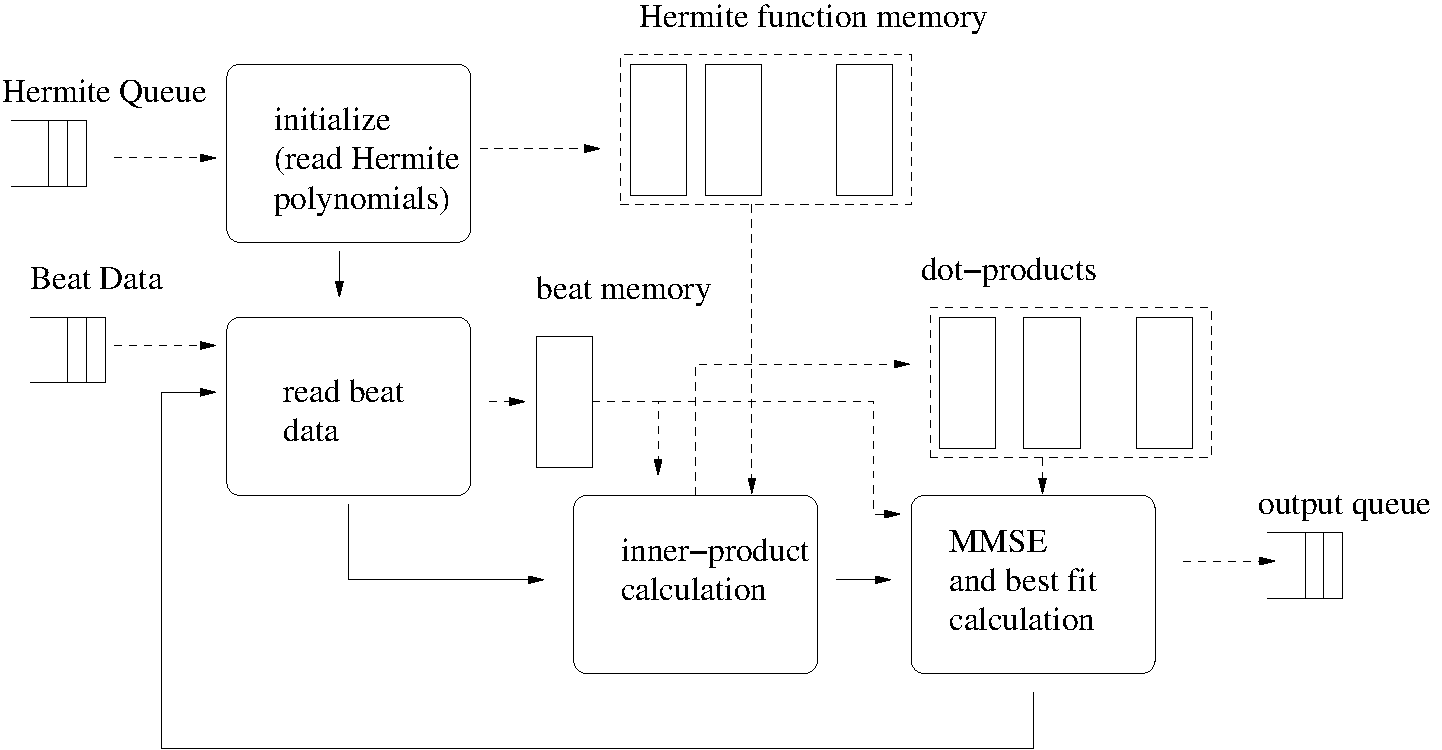
\includegraphics[width=\linewidth]{HardwareArchitecture.pdf}
	\caption{Hardware Architecture}
	\label{fig:HardwareArchitecture}
\end{center}
\end{figure}

The VHDL hardware for this design is generated using the AHIRV2 toolchain
which was described in Section \ref{s:AHIRV2}.  
The generated VHDL is instantiated in the FPGA together with the RIFFA wrappers,
and the resulting design is synthesized and mapped to the Virtex-6 FPGA using
the Xilinx ISE 14.3 toolset.


%
%HDL for this design is generated using AHIR HLS toolchain. It is equipped with a library 
%of heavily pipelined Floating Point operators and Loop Pipelining mechanism which 
%enables the final VHDL to extract parallelism in C program. It uses pipes to communicate 
%between testbench and the program, which translate to FIFOs in hardware. A simple integration 
%interface between these FIFOs and RIFFA channels completes the system. 
%
%
%The RIFFA software drivers and interface infrastructure is used to communicate between 
%host and FPGA card \cite{c:jacobsen13}. It supports upto 12 independent
%channels for data transmission. All of them end in separate Rx/Tx FIFOs on FPGA that 
%can operate on different clock domains at either ends. A simple integration 
%interface bridges RIFFA and AHIR generated FIFOs.
%By incorporating functions provided by RIFFA driver, same testbench used for 
%Software verification can be used for verifying the hardware.
%  Describe the 
%    - overall system.
%    - card
%    - the driver
%    - the hardware generation process.
%

\section{Results}\label{s:results}

We measure the round-trip delay and FPGA core power consumption for processing one beat. 
The round-trip delay is the time interval between the beginning of transmission of 
beat-data from the host to the hardware and the beginning of reception of best fit
coefficients from the hardware. 
The test feeds a single beat at a time to the FPGA and measures the latency.

In the implementation, the two outer-loops described in Sections \ref{sec:InnerProduct} and
 \ref{sec:MMSE} were unrolled to different
extents to see the impact of unrolling on the system performance. 
Three levels of unrolling were tried: one-way, two-way and four-way.  
The four-way unrolling gave the best performance,
as expected.  The results are summarized in Table \ref{table:Results} (the reported latency
is the average value observed across 100 beats).  
The minimum latency achieved with four-way-unrolling was observed to be
$0.39$ ms (for the processing of a single 144-sample beat).
The power dissipation values are
measured using hardware monitoring while the beats are being processed, and represent peak
power dissipation.

%%%%%%%% Results Table %%%%%%%%%%%%%
\begin{table}[ht]
\caption{Results:  FPGA utilization and latency for different loop-unrolling levels} %title
\centering
\begin{tabular}{c @{\hskip 0.05in}| @{\hskip 0.05in}c@{\hskip 0.15in}c @{\hskip 0.15in} c @{\hskip 0.15in} c} %5 centered columns
\hline\hline\\[-1.5ex]

Unroll-level & \begin{tabular}[c]{@{}c@{}}Slice LUT  \\ Utilization  \end{tabular}& \begin{tabular}[c]{@{}c@{}}Slice Register  \\Utilization  \end{tabular}& \begin{tabular}[c]{@{}c@{}}Avg. Processing  \\Latency \end{tabular} & \begin{tabular}[c]{@{}c@{}}FPGA core Power \\ Consumption \end{tabular}\\ [2ex] \hline \\[-1.5ex]%heading

1-way & 56839 & 65995 & 1.39ms & 2.75W \\

2-way & 65895 & 80709 & 0.80ms & 2.88W \\

4-way & 84331 & 110165 & 0.44ms & 3.09W \\ [1ex]

\hline
\end{tabular}
\label{table:Results}
\end{table}
%%%%%%%%%%%%%%%%%%%%%%%%%%%

It is clear that FPGA can be used for {\em true} real-time processing since the 
computation time required to process a pair of beats (corresponding
to a heart-beat sampled on two channels) is less than $1ms$, which is
much smaller than time-interval between actual heart beats (which is about $1s$). 
The observed power dissipation is 3.1W.  Hardware utilization in 4-way unrolled 
system is less than $55\%$ of the FPGA resource.

\subsection{Comparison with GPU/CPU implementations}

Hermite basis fitting has been evaluated on GPU and CPU implementations
as well.  For example, in \cite{c:GPU}, the authors demonstrate a
GPU implementation that shows excellent scaling behaviour in real-time, so that 
100K beats can be processed in 15.7 seconds. The average processing latency per 
pair of beats if 0.022 msecs.  However, it must be stressed that in general the GPU achieves 
full parallelization when a huge set of data is processed and real-time requires the processing 
of small sets of data. Real-time is achieved on the GPU by means of processing chunks of 10 and 100 beats, 
resulting in latencies of around 10 seconds and around 100 seconds respectively. Thus, 
{\em true} real-time processing is not fully acomplished since latencies are too long. 
On the other hand, a CPU is able to do low-latency real-time wih a latency per beat of around 
30 msecs per pair of beats.  As for our FPGA implementation, the latency needed to process a pair of beats 
is under $1ms$. Since the beats are processed one at a time, actual real-time is achieved. 

These comparisons are made against the same algorithm executed on Intel-i7 PC(1.6GHz) 
and NVIDIA TESLA C2050 (1.15GHz) \cite{c:GPU}. The operating frequency on the FPGA
card was 100MHz which is less than one-tenth of that used on CPUs and GPUs.
Further, the peak power consumption (while actually processing the beats) on the FPGA is $3W$ as compared to 
$100W+$ on Core i7 processors and $200W+$ on the GPU.  %% which GPU?
In summary, the FPGA achieves a better average latency than the CPU and it ourperforms the 
GPU in term of the low-latency requirements for \textit{actual} real-time capabilities, 
displaying a power comsumption which is two orders of magnitude lower than the other two technologies. 
Thus, the FPGA is an attractive option for low energy real-time ECG classification
applications in portable health monitoring devices.

\section{Conclusions}\label{s:conclusions}

In this paper, a solution to the problem of Hermite polynomial
based heart-beat characterization using FPGAs is presented.
We have mapped the problem to hardware using algorithm-to-hardware
techniques (with the AHIRV2 tools).  The Xilinx ML605 card with a
Virtex-6 FPGA was used as the platform and the RIFFA host-interface was used to
communicate with the FPGA card. 

This methodology is presented as an alternative to existing software oriented approaches, 
for real-time latency-sensitive signal processing. When using the FPGA, a substantial
latency reduction in single-beat processing was observed (in comparison with both
GPU and CPU implementations of the same algorithm).  
Further, the peak power dissipation in
the FPGA is almost two orders of magnitude lower than that observed in the CPU/GPU case.

The highly parallel GPU and CPU architectures are very effective in off-line processing
(processing of a large number of beats, not necessarily in real-time).  When it comes to real-time,
online beat processing, our work demonstrates that dedicated hardware implementation
using an FPGA offers a very competitive platform for ECG signal processing.




% conference papers do not normally have an appendix


% use section* for acknowledgement

\section*{Acknowledgment}

The authors would like to thank Rakesh Mehta for providing access to
the Xilinx ML605 FPGA board.




% trigger a \newpage just before the given reference
% number - used to balance the columns on the last page
% adjust value as needed - may need to be readjusted if
% the document is modified later
%\IEEEtriggeratref{8}
% The "triggered" command can be changed if desired:
%\IEEEtriggercmd{\enlargethispage{-5in}}

% references section

% can use a bibliography generated by BibTeX as a .bbl file
% BibTeX documentation can be easily obtained at:
% http://www.ctan.org/tex-archive/biblio/bibtex/contrib/doc/
% The IEEEtran BibTeX style support page is at:
% http://www.michaelshell.org/tex/ieeetran/bibtex/
%\bibliographystyle{IEEEtran}
% argument is your BibTeX string definitions and bibliography database(s)
%\bibliography{IEEEabrv,../bib/paper}
%
% <OR> manually copy in the resultant .bbl file
% set second argument of \begin to the number of references
% (used to reserve space for the reference number labels box)

\bibliographystyle{IEEEbib}
\bibliography{refsQRS}

%\begin{thebibliography}{1}
%
%\bibitem{IEEEhowto:kopka}
%H.~Kopka and P.~W. Daly, \emph{A Guide to \LaTeX}, 3rd~ed.\hskip 1em plus
%  0.5em minus 0.4em\relax Harlow, England: Addison-Wesley, 1999.
%
%\end{thebibliography}




% that's all folks
\end{document}



